\chapter{Tests and results}\label{ch:test}
Testing of the drone involves, testing the drone stabilization and hovering its manual control and landing. But before a flight test is done, the drone must be tested  to verify if all its sensors are in order and it also requires an initial calibration of the sensors. The sensors are run in a multi-core architecture, where the i2c devices run on core 1, motors and receivers run on core 2 and GPS and telemetry run on core 3. When running individual sensor tests, dummy functions are introduced to occupy the vacant cores. The tests that are provided for every sensor are as follows:
\begin{enumerate}
    \item Motor test - This test is used to check the direction and the order of the motors as shown in Fig. \ref{fig:motor_direction}. In this test, the motors spin sequentially in an order for 5 seconds each.
     \item ESC calibration test - This test is necessary when a new ESC is used. The 4 ESCs are calibrated to start the motors at 1000$\mu$s pulse and reach its maximum at 2000$\mu$s pulse. This is done by:
     \begin{itemize}
         \item Turn on the transmitter and put the throttle at the maximum position
         \item Switch on the FPGA and upload the program
         \item Wait for the motors to beep 3 times in sets of 3, then lower the throttle of transmitter and wait for the motors to beep again.
         \item Motors are calibrated successfully
     \end{itemize}
    \item IMU test - This test is used to verify the direction and magnitude of pitch, roll and yaw angles of the quad-rotor. The directions of the angles are given in Fig. \ref{fig:imu_angle}. The directions follow right hand thumb rule. Therefore, roll is positive when left wing goes up, pitch is positive when the nose pitches up and yaw is positive when the drone rotates to the right.
    \item Barometer test - This test is used to check the readings of barometer whether they decrease as the drone goes up and increase as the drone descends since, the atmospheric pressure increases with decrease in altitude.
    \item Compass test - This test is used to check the yaw of the drone with respect of the absolute north. The yaw angles are then rounded off to stay in between 0 to 360.
     \item Receiver test - 
     \textit{NOTE: Check if the receiver is paired to transmitter before starting this test [\ref{trans_receiver_pair}]}. 
     This test is used to check if all the channels of the transmitter are being read by the FPGA. The direction and the value limits of the transmitter channels are also calculated and added as transmitter settings to the header file of the Flight controller code. For every channel the minimum, maximum and its middle value are recorded and the direction of the transmitter channel required are displayed in Fig. \ref{fig:tranmitter_direction}. If the direction is opposite to the required direction, the reverse variable of the particular channel is set to 1.
     \item GPS test - This test is used to verify that the GPS has a 3D position lock, i.e. the GPS is locked to more than 8 satellites and displays the current GPS coordinates.
     \item Telemetry test - \textit{NOTE: check is the baud rate for the telemetry is set to 115200 [\ref{telemetry_baud}]}. This test code is used to send and receive telemetry data between different telemetry modules. The test code sends a "hello world" message, and the user runs a python script called  \textit{telemetry\_base} to receive the sent data.
     The test code also contains a code to help tune the PID gains of the motors real time by sending the gain values to the drone wirelessly. This program although can send and receive the gain values, the tuning was unsuccessful real time because, the loop runs at a much lower frequency than the main loop.
     \item Analog test - The test sends a configuration word which specifies how the module has to read the input(either a differential or an absolute input value). In every iteration it changes the module configuration word, so the test program obtains a read from all the analog input pins on the ADC in differential and absolute modes.
\end{enumerate}

\begin{figure} [ht]
    \centering
    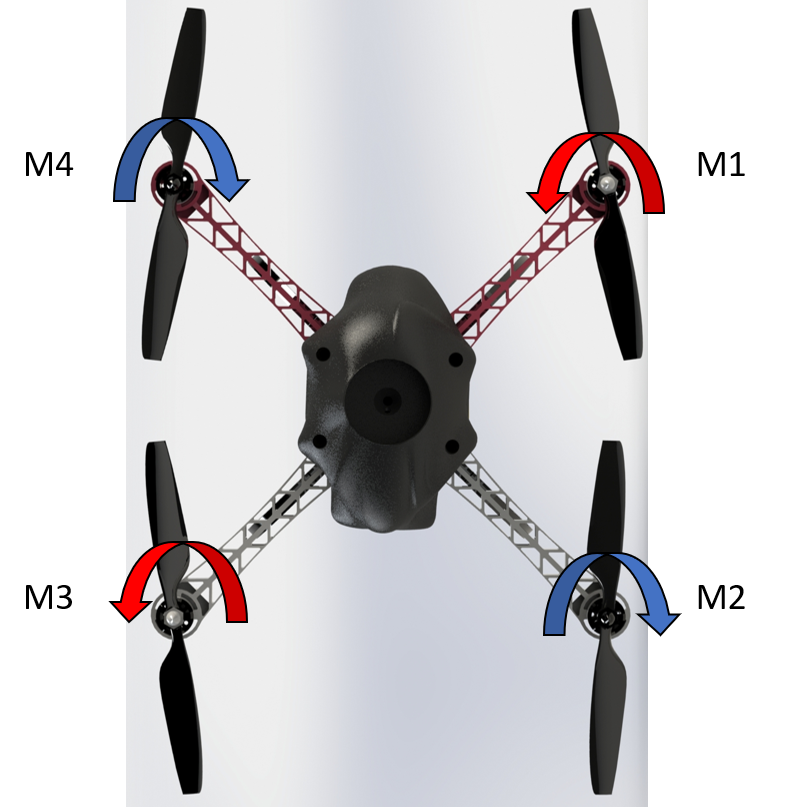
\includegraphics[width=0.5\textwidth]{Figures/testing/motor_directions.png}
    \caption{Directions and order of the motor Assembly}
    \label{fig:motor_direction}
\end{figure}

\begin{figure} [ht]
    \centering
    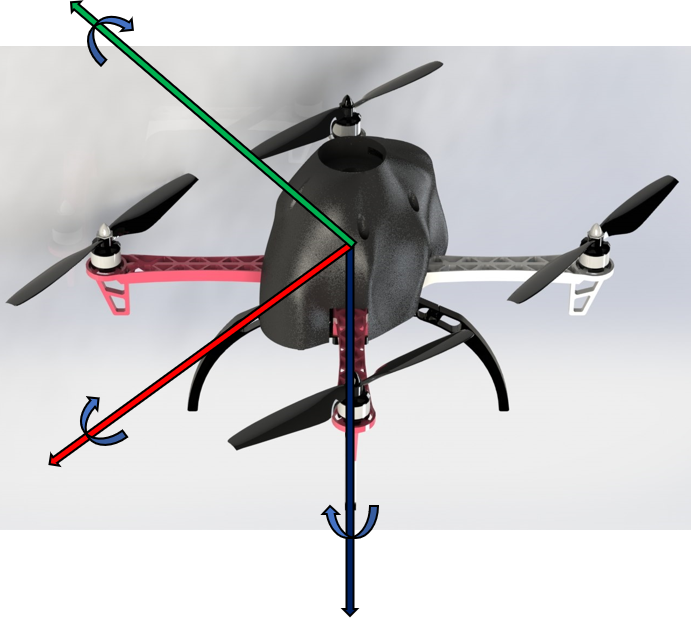
\includegraphics[width=0.5\textwidth]{Figures/testing/imu_directions.png}
    \caption{Roll (X axis, on red), pitch (Y axis, on green) and yaw (Z axis, on black) angles, and the directions of the drone.}
    \label{fig:imu_angle}
\end{figure}

\begin{figure} [ht]
    \centering
    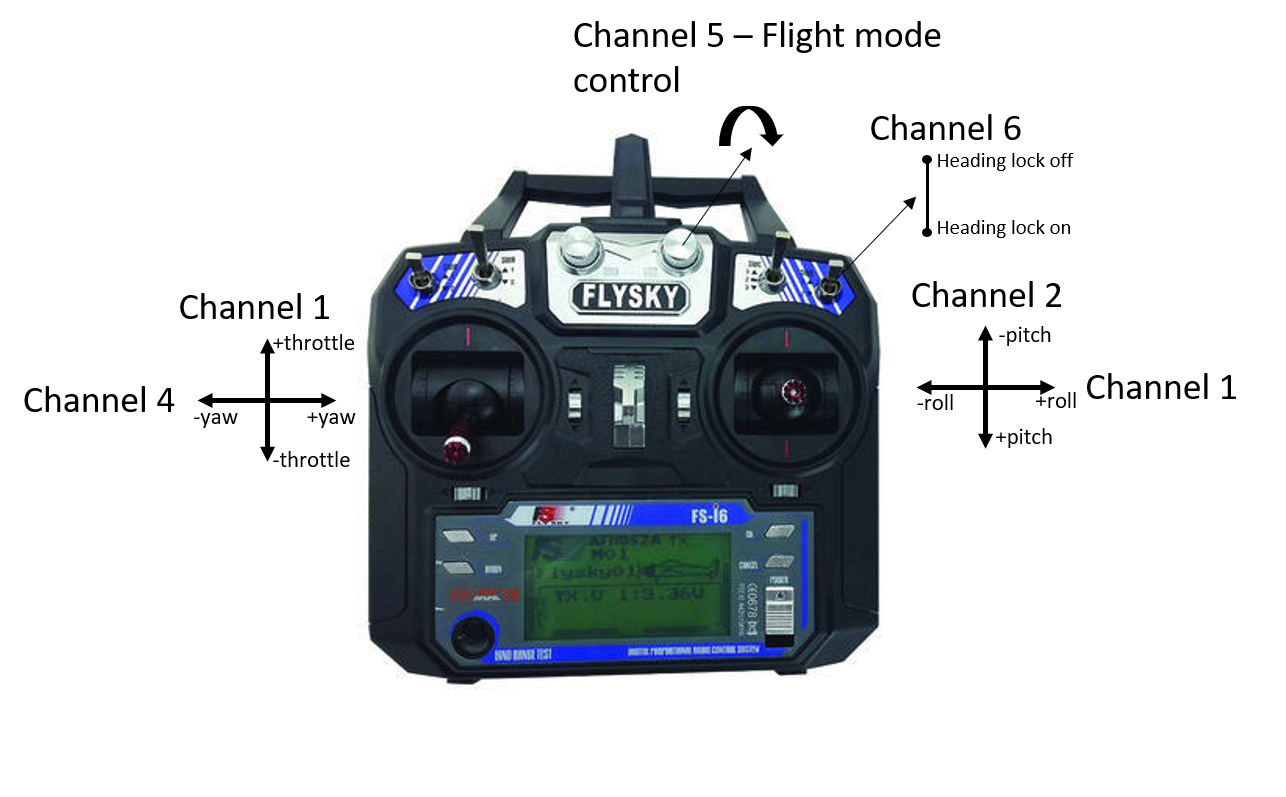
\includegraphics[width=0.5\textwidth]{Figures/testing/transmitter_controls.png}
    \caption{The configurations of a 6-channel transmitter}
    \label{fig:tranmitter_direction}
\end{figure}

After the sensors have been tested, it is necessary to tune the PID values of roll, pitch and yaw angles.



\section{PID tuning test}\label{app:tuning}
The PID tuning procedure is followed as described in \cite{bib:brooking}. The PID gains are tuned while holding the drone at hovering throttle:
\begin{enumerate}
    \item The drone is kept on a flat ground (preferably on grass or carpet) and the initial yaw PID values are set to $K_P=1$,$K_D=0.001$ and $K_i=0$ so as to prevent the drone from rotating while tuning roll and pitch.
    \item The roll and pitch are assumed to have similar gains. The $K_P$ and $K_i$ values are set to 0 and only $K_D$ is varied. 
    \item This values is increased until the drone just becomes restless. The final $K_D$ is taken as 75\% of the current value.
    \item The $K_P$ gain is now increased in steps of 0.2 until it just begins to oscillate. The final $K_P$ is taken as 50\% of the current value.
    \item Similarly, the $K_i$ gain is increased in steps of 0.0001 until it just begins to oscillate. The final $K_i$ is taken as 50\% of the current value.
\end{enumerate} 


\section{Flight test}
Once the PID values are tuned, the manual control of the drone is tested. The test was done in the Vicon lab at AAU. The drone was made to takeoff and the motions of the drone was controlled using a transmitter as seen in Figures \ref{fig:test_floor} and \ref{fig:test_fly}.

Although the barometer sensor was tested for altitude hold mode, the altitude PID values were not tuned due to time constraints. Due to this, the drone takes off and can be controlled but cannot be used in hover mode. Also due to the same reason, it gets difficult while landing the drone. But the cover protects the components from being damaged and due to the height of the cover, it also protects the propellers from over damage as seen in Figure \ref{fig:test_lmao}.

\begin{figure} [!ht]
    \centering
    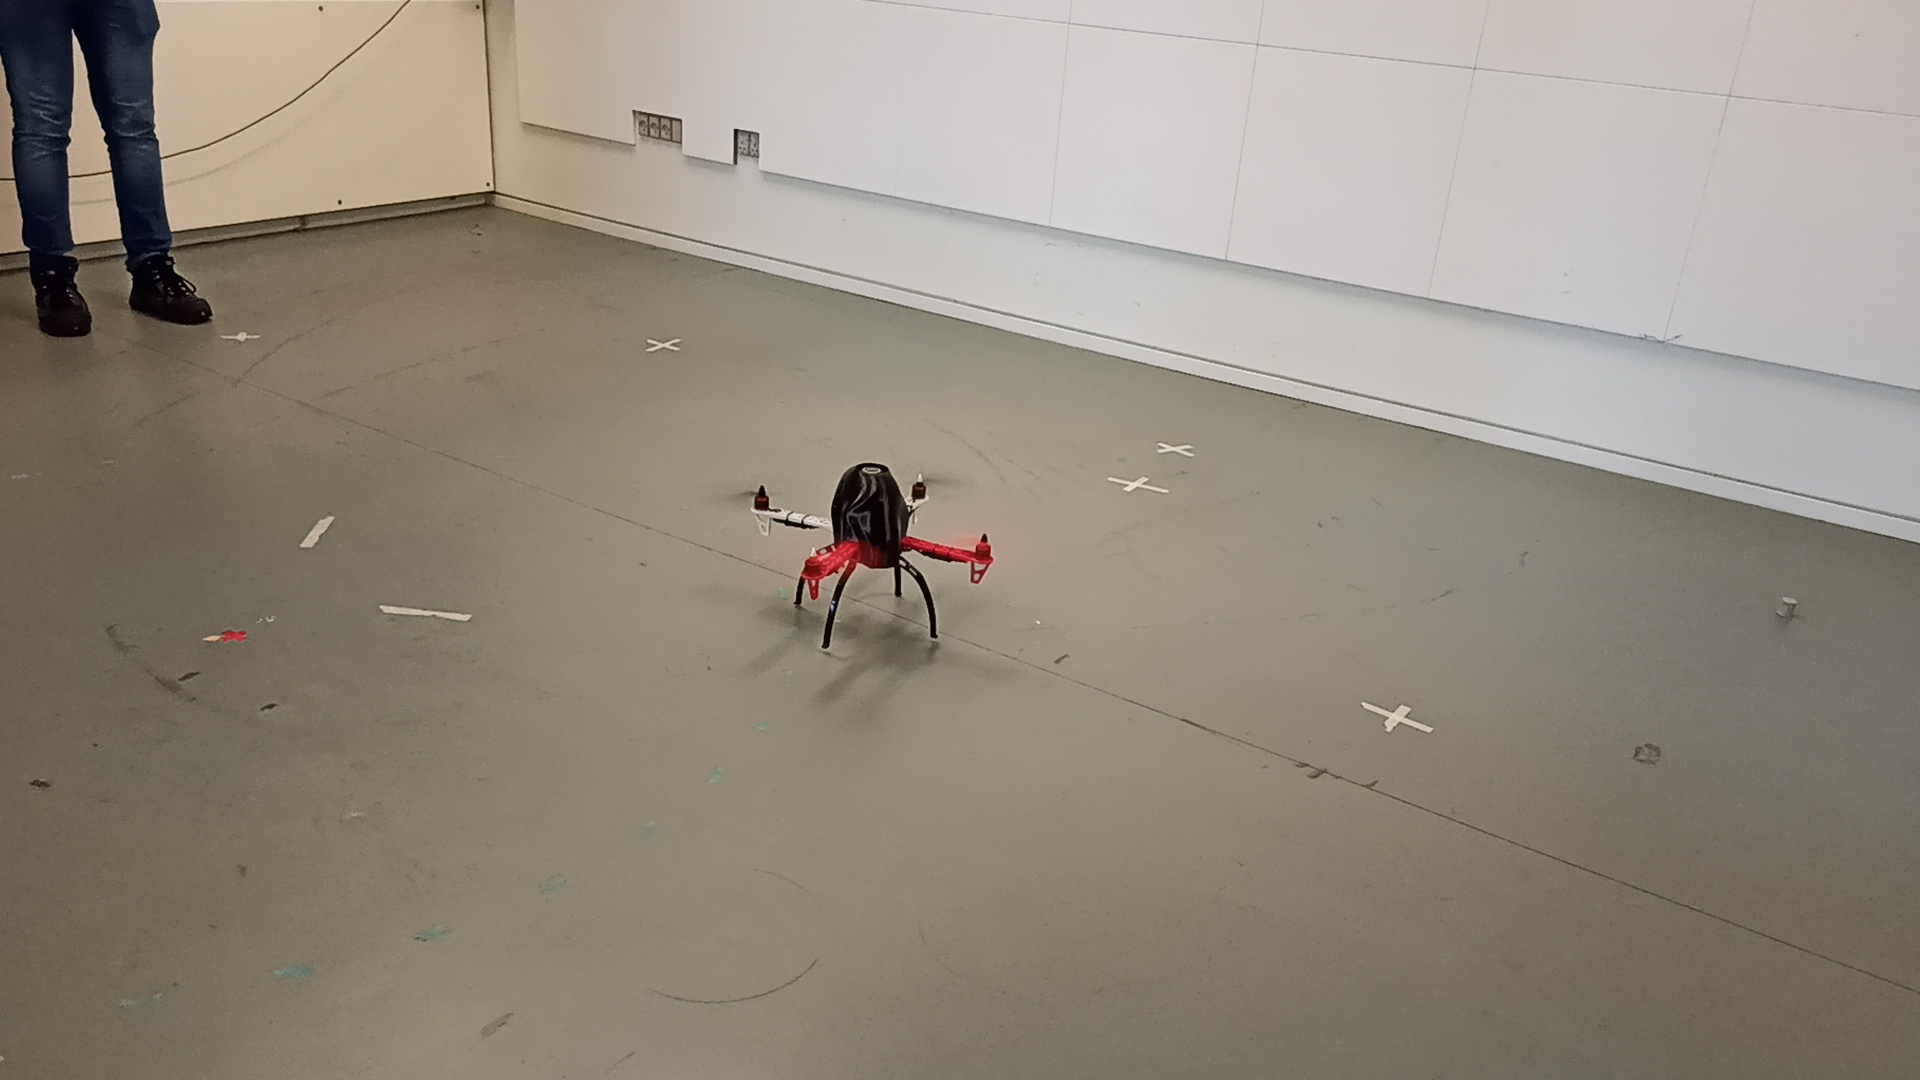
\includegraphics[width=\textwidth]{Figures/testing/drone_floor.jpg}
    \caption{Drone 1 (Model-A) about to take off}
    \label{fig:test_floor}
\end{figure}


\begin{figure} [!ht]
    \centering
    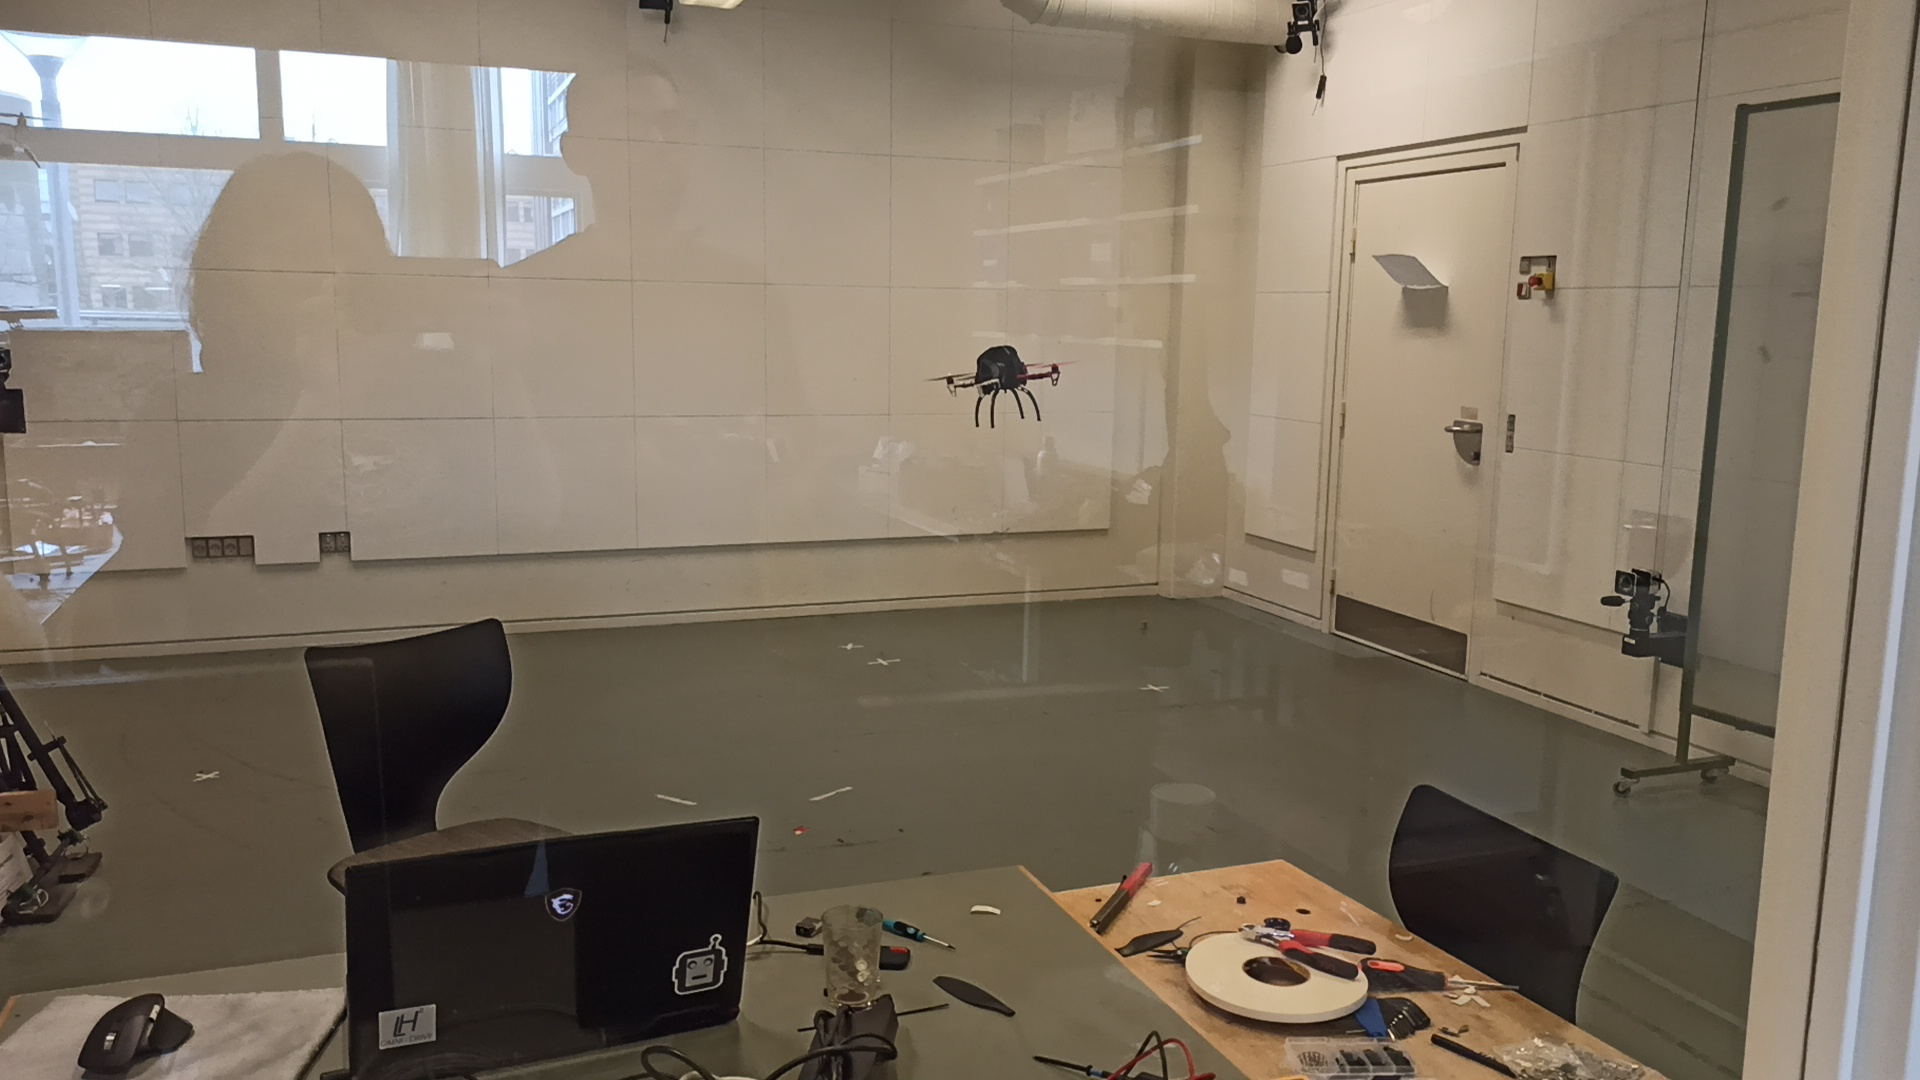
\includegraphics[width=\textwidth]{Figures/testing/drone_flying_lab.jpg}
    \caption{Manual control of the drone}\label{fig:test_fly}
\end{figure}


\begin{figure} [!ht]
    \centering
    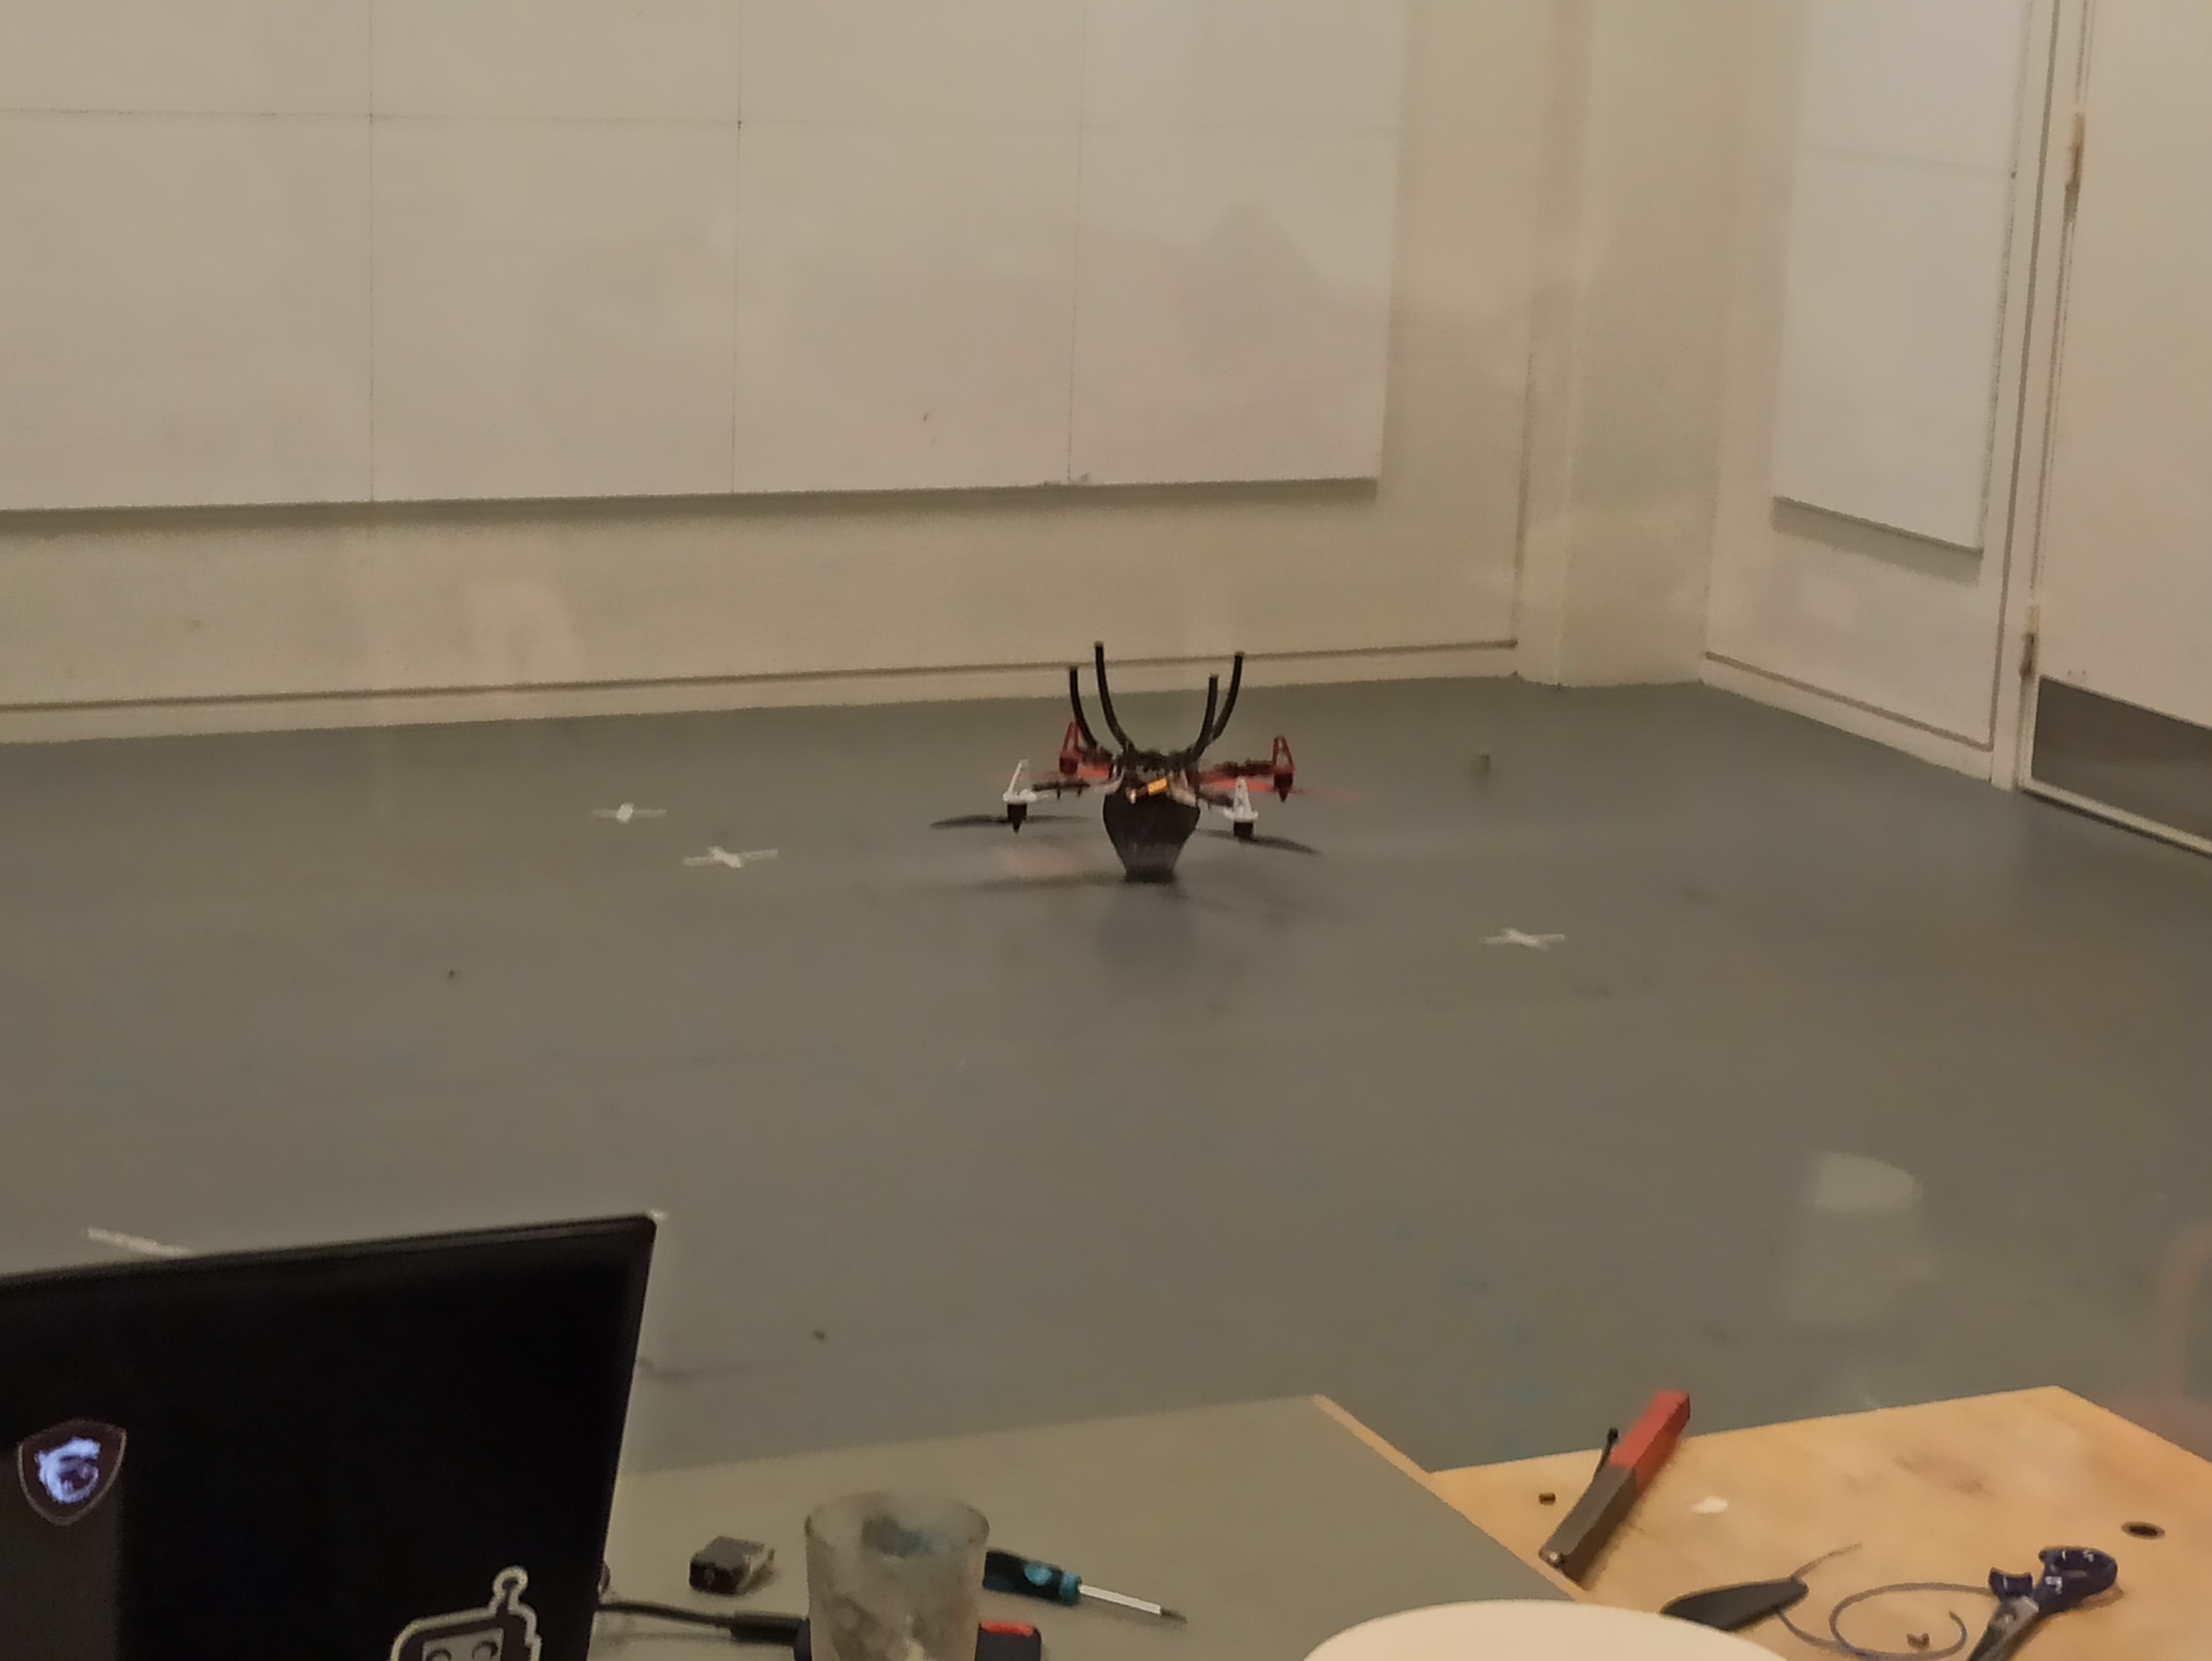
\includegraphics[width=\textwidth]{Figures/testing/SURPISEEE.jpg}
    \caption{The cover is able to protect the propellers when landing upside down.}\label{fig:test_lmao}
\end{figure}